% ------------------------------------------------------------------------------
% TYPO3 Version 10.2 - What's New (Serbian Version)
%
% @license	Creative Commons BY-NC-SA 3.0
% @link		http://typo3.org/download/release-notes/whats-new/
% @language	Serbian
% ------------------------------------------------------------------------------

\section{Administratorski interfejs}
\begin{frame}[fragile]
	\frametitle{Administratorski interfejs}

	\begin{center}\huge{Poglavlje 1:}\end{center}
	\begin{center}\huge{\color{typo3darkgrey}\textbf{Administratorski interfejs}}\end{center}

\end{frame}

% ------------------------------------------------------------------------------
% Feature | 89458 | Show link to online docs in extension manager

\begin{frame}[fragile]
	\frametitle{Administratorski interfejs}
	\framesubtitle{Extension Manager}

	Extension Manager prikazuje linkove ka dokumentaciji proširenja.

	\begin{figure}
		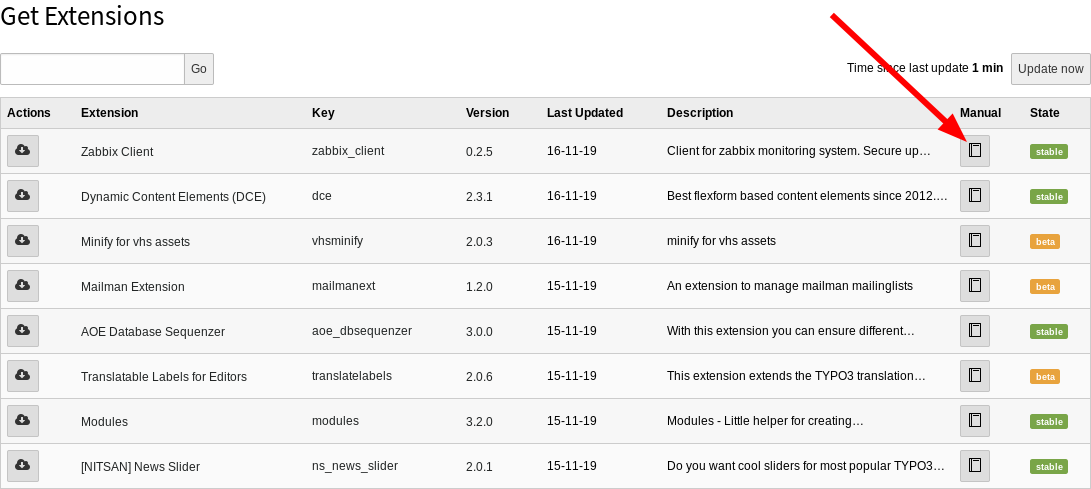
\includegraphics[width=0.90\linewidth]{ChangesForIntegrators/89458-ShowLinkToOnlineDocsInExtensionManager.png}
	\end{figure}

\end{frame}

% ------------------------------------------------------------------------------
% Feature | 86818 | Reintroduce keyboard accessible version of the pagetree

\begin{frame}[fragile]
	\frametitle{Administratorski interfejs}
	\framesubtitle{Pristup stablu strana}

	Korisnici administratorskog interfejsa mogu da koriste tastaturu da se kreću
	kroz stablo strana. Na primer sa strelicama, "home", "end", "enter", "space", i tako dalje.
	\newline
	Ovo je u skladu sa najboljim praksama kao što je opisano u
	\href{https://www.w3.org/TR/wai-aria-practices-1.1/#keyboard-interaction-22}{WAI-ARIA Authoring Practices 1.1}
	od strane W3C.

	\begin{figure}
		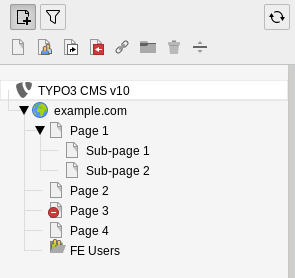
\includegraphics[width=0.30\linewidth]{BackendUserInterface/86818-PagetreeAccessibility.png}
	\end{figure}

\end{frame}

% ------------------------------------------------------------------------------
